%% This Beamer template is based on the one found here: https://github.com/sanhacheong/stanford-beamer-presentation, and edited to be used for Stanford ARM Lab

\documentclass[10pt]{beamer}
%\mode<presentation>{}

\usepackage[spanish]{babel}
\usepackage{media9}
\usepackage{amssymb,amsmath,amsthm,enumerate}
\usepackage[utf8]{inputenc}
\usepackage[T1]{fontenc}
\usepackage{array}
\usepackage[parfill]{parskip}
\usepackage{graphicx}
\usepackage{caption}
\usepackage{subcaption}
\usepackage{bm}
\usepackage{amsfonts,amscd}
\usepackage[]{units}
\usepackage{listings}
\usepackage{multicol}
\usepackage{multirow}
\usepackage{tcolorbox}
\usepackage{physics}
\usepackage{circuitikz}
\usepackage{wrapfig}

% Enable colored hyperlinks
%\hypersetup{colorlinks=true}

% The following three lines are for crossmarks & checkmarks
\usepackage{pifont}% http://ctan.org/pkg/pifont
\newcommand{\cmark}{\ding{51}}%
\newcommand{\xmark}{\ding{55}}%

% Numbered captions of tables, pictures, etc.
\setbeamertemplate{caption}[numbered]

%\usepackage[superscript,biblabel]{cite}
\usepackage{algorithm2e}
\renewcommand{\thealgocf}{}

% Bibliography settings
\usepackage[style=ieee]{biblatex}
\setbeamertemplate{bibliography item}{\insertbiblabel}
\addbibresource{references.bib}

% Glossary entries
\usepackage[acronym]{glossaries}
\newacronym{ML}{ML}{machine learning}
\newacronym{HRI}{HRI}{human-robot interactions}
\newacronym{RNN}{RNN}{Recurrent Neural Network}
\newacronym{LSTM}{LSTM}{Long Short-Term Memory}


\theoremstyle{remark}
\newtheorem*{remark}{Remark}
\theoremstyle{definition}

\newcommand{\empy}[1]{{\color{darkorange}\emph{#1}}}
\newcommand{\empr}[1]{{\color{cardinalblue}\emph{#1}}}
\newcommand{\examplebox}[2]{
  \begin{tcolorbox}[colframe=darkcardinal,colback=boxgray,title=#1]
	#2
\end{tcolorbox}}

\usetheme{Stanford} 
\def \i  {\item}
\def \ai {\item[] \quad \arrowbullet}
\newcommand \si[1]{\item[] \quad \bulletcolor{#1}}
\def \wi {\item[] \quad $\ \phantom{\Rightarrow}\ $}
\def \bi {\begin{itemize}\item}
\def \ei {\end{itemize}}
\def \be {\begin{equation*}}
\def \ee {\end{equation*}}
\def \bie {$\displaystyle{}
\def \eie {{\ }$}}
\def \bsie {\small$\displaystyle{}
\def \esie {{\ }$}\normalsize\selectfont}
\def \bse {\small\begin{equation*}}
\def \ese {\end{equation*}\normalsize}
\def \bfe {\footnotesize\begin{equation*}}
\def \efe {\end{equation*}\normalsize}
\renewcommand \le[1] {\\ \medskip \lefteqn{\hspace{1cm}#1} \medskip}
\def \bex {\begin{example}}
\def \eex {\end{example}}
\def \bfig {\begin{figure}}
\def \efig {\end{figure}}
\def \btheo {\begin{theorem}}
\def \etheo {\end{theorem}}
\def \bc {\begin{columns}}
\def \ec {\end{columns}}
\def \btab {\begin{tabbing}}
\def \etab {\end{tabbing}\svneg\svneg}
\newcommand \col[1]{\column{#1\linewidth}}
\def\vneg  {\vspace{-5mm}}
\def\lvneg {\vspace{-10mm}}
\def\svneg {\vspace{-2mm}}
\def\tvneg {\vspace{-1mm}}
\def\vpos  {\vspace{5mm}}
\def\lvpos {\vspace{10mm}}
\def\svpos {\vspace{2mm}}
\def\tvpos {\vspace{1mm}}
\def\hneg  {\hspace{-5mm}}
\def\lhneg {\hspace{-10mm}}
\def\shneg {\hspace{-2mm}}
\def\thneg {\hspace{-1mm}}
\def\hpos  {\hspace{5mm}}
\def\lhpos {\hspace{10mm}}
\def\shpos {\hspace{2mm}}


% commands to relax beamer and subfig conflicts
% see here: https://tex.stackexchange.com/questions/426088/texlive-pretest-2018-beamer-and-subfig-collide
\makeatletter
\let\@@magyar@captionfix\relax
\makeatother

\title[Proyecto Final]{Estudio e implementación de un administrador de baterías de Litio-ion}
\subtitle{Presentación de Avances}

%\beamertemplatenavigationsymbolsempty

\begin{document}

\institute{
  \vskip 5pt
  \begin{figure}
	\centering
	\begin{subfigure}[t]{0.5\textwidth}
	  \centering
	  
\includegraphics[height=0.7in]{./images/LOGO-UNR-NEGRO.png}
	\end{subfigure}%
	~ 
	\begin{subfigure}[t]{0.5\textwidth}
	  \centering
	  
\includegraphics[height=0.5in]{./images/FCEIA-logo.png}
	\end{subfigure}
  \end{figure}
  \vskip 5pt
  Facultad de Ciencias Exactas, Ingeniería y Agrimensura\\
  Universidad Nacional de Rosario\\
  \vskip 1pt
}

\author[Escuela de Ingeniería Electrónica]{
  \begin{tabular}{ccc} 
	Federico Ceccarelli & Martin Moya & Lucio Santos\\
	\footnotesize
	\texttt{\href{mailto:fededc88@gmail.com}{fededc88@gmail.com}} &
	\footnotesize
	\texttt{\href{mailto:moyamartin1@gmail.com}{moyamartin1@gmail.com}} &
	\footnotesize
	\texttt{\href{mailto:lucio.santos2206@gmail.com}{lucio.santos2206@gmail.com}}
  \end{tabular}
\vspace{-4ex}}



\date{\today}

\begin{noheadline}
  \begin{frame}\maketitle\end{frame}
\end{noheadline}

\setbeamertemplate{itemize items}[default]
\setbeamertemplate{itemize subitem}[circle]

\begin{frame}[allowframebreaks]
  \frametitle{Contenidos} % Table of contents slide, comment this block out to remove it
  \tableofcontents % Throughout your presentation, if you choose to use \section{} and \subsection{} commands, these will automatically be printed on this slide as an overview of your presentation
\end{frame}

\section{Avances}
\begin{frame}[allowframebreaks]
  \frametitle{Avances del Proyecto}
  \begin{itemize}
	\item Selección del Sensor de corriente
	\item Diseño de un modelo de una celda de Litio-Ion
	\item Estimación del estado de carga utilizando un Filtro de Kalman
  \end{itemize}
\end{frame}

\section{Sensor de Corriente}

\begin{frame}[allowframebreaks]
  \frametitle{Sensor de Corriente}
  \begin{minipage}{0.4\textwidth}
	\textbf{Objetivos}
	\small
	\begin{itemize}
	  \item Mantener al pack operando dentro del SOA.
	  \item Monitorear la distribución de carga entre celdas
	  \item Implementar y mantener un seguimiento preciso del SoC
	  \vspace{4\baselineskip}
	\end{itemize}
  \end{minipage}
  \hfill
  \begin{minipage}{0.4\textwidth}
	\textbf{Tecnologías disponibles}
	\small
	\begin{itemize}
	  \item \textbf{Resistencia Shunt}
	  \item Transformador de Intensidad
	  \item \textbf{Sensor de Efecto Hall}
	  \item Sensor de Impedancia Magnética
	  \item Sensor de Magnetoresistencia Gigante
	  \item Sensores Ópticos
	\end{itemize}
  \end{minipage}
  
\end{frame}

\begin{frame}[allowframebreaks]
  \frametitle{Tecnologías disponibles}

\end{frame}

\begin{frame}[allowframebreaks]
  \frametitle{Resistencia Shunt}
  Calcula la corriente de forma indirecta midiendo la caída de tensión sobre
  una resistencia, que tiene un valor del órden de los miliohmios, al circular
  la corriente incógnita. Su esquemático se puede observar en la Figura
  \ref{sch_shunt}.

  \begin{figure}[h!]
	\begin{circuitikz}\draw
	  (0, 0) to[resistor=$R_{shunt}$, i_>=$I$] (6, 0)
	  ;
	  \draw
	  (2, 0) to[short, *-] (2, 1.5)
	  (2, 1.5) to[voltmeter] (4, 1.5)
	  (4, 1.5) to[short, -*] (4, 0)
	  ;
	\end{circuitikz}
	\caption{Esquemático de un sensor de corriente por resistencia shunt}
	\label{sch_shunt}
  \end{figure}

  \framebreak

  Características y consideraciones:
  \begin{itemize}
	\item Alta relación de costo-efectividad, empaquetado compacto y aplicable
	  en mediciones tanto de corriente continua como alterna.
	\item Alta frecuencia de corte (decenas de MHz).
	\item Carece de aislación galvánica.
	\item Alto rango de temperatura de operación.
	\item La resistencia shunt presenta una inductancia intrínseca,
	  comprometiendo el ancho de banda y la presición
  \end{itemize}
\end{frame}
% This demonstrates a new section

\begin{frame}[allowframebreaks]
  \frametitle{Sensor de Efecto Hall}
  \begin{figure}[h!]
	\begin{minipage}{0.45\textwidth}
	  \begin{itemize}
		\item Sensor de efecto magnético basado en el fenómeno físico denominado
		  \emph{Efecto Hall}.
		\item Dispositivo aislado, no intrusivo. Mide CA como CC. Su esquemático
		  se puede observar en la Figura \ref{sch_hall}
	  \end{itemize}
	\end{minipage}
	\hspace{10pt}
	\begin{minipage}{0.45\textwidth}
	  \centering
	  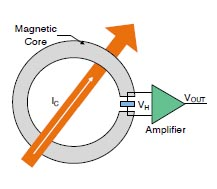
\includegraphics[width=0.8\textwidth]{./images/Open-loop_Hall_Sensor.jpg}
	  \caption{Esquemático de un sensor de Efecto Hall}
	  \label{sch_hall}
	\end{minipage}
  \end{figure}

  \textbf{Consideraciones}:
  \begin{itemize}
	\item Debido al efecto de saturación magnética del núcleo, posee
	  limitaciones en picos de corriente y frecuencias menores al MHz.
	\item Sensible a la influencia de los campos magnéticos externos.
	\item Presenta un voltaje de offset que es poco estable y varía
	  fuertemente a cambios de temperatura.
  \end{itemize}
\end{frame}

\begin{frame}[allowframebreaks]
  \frametitle{Tecnología seleccionada}
  Dada la naturaleza del BMS, elegimos el método de medición de corriente por
  resistencia Shunt, ya que posee las siguientes ventajas:

  \begin{itemize}
	\item Bajo offset y baja susceptibilidad frente a campos magnéticos externos
	  y variaciones de temperatura.
	\item Alta linealidad, mayormente cerca de la zona cercana al cero y a la
	  saturación del núcleo, como también ante altas temperatura (bajo TCR).
	\item Mejor resolución para mediciones de corriente continua, debido a la
	  baja sensitividad ante los campos magnéticos.
	\item Fácil integración en circuitos impresos.
	\item Disponibilidad de distribuidores nacionales.
  \end{itemize}

\end{frame}


\begin{frame}
  \frametitle{Sensor de Corriente - INA226}
  El sensor a utilizar es el INA226 de la marca \emph{Texas Instruments} que
  posee las siguientes características:
  \begin{itemize}
	\item ADC de 16 bits
	\item Interfaz I/O compatible con I2C.
	\item Implementa un multiplicador/divisor interno, esto permite pre-calcular
	  la corriente y potencia de forma rápida.
  \end{itemize}

%  \framebreak

  \begin{figure}[h!]  
   \centering
	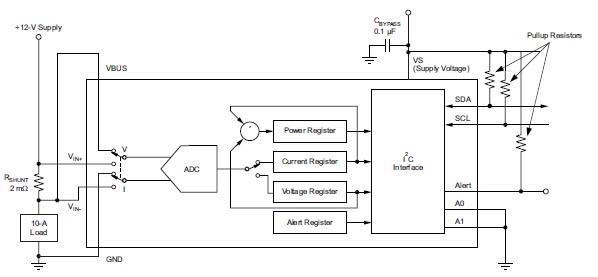
\includegraphics[width=0.75\linewidth]{./images/INA226-Common_Implementation.jpg}
	\caption{Implementación del INA226}
	\label{sch_ina226}	
  \end{figure}

\end{frame}


\section{Celda de Litio-Ion NCR18650PF}

\begin{frame}
  \frametitle{Celda NCR18650PF}

  \vspace{10pt}
  \begin{figure}[h!]
	\begin{minipage}{0.3\textwidth}
	  \centering
	  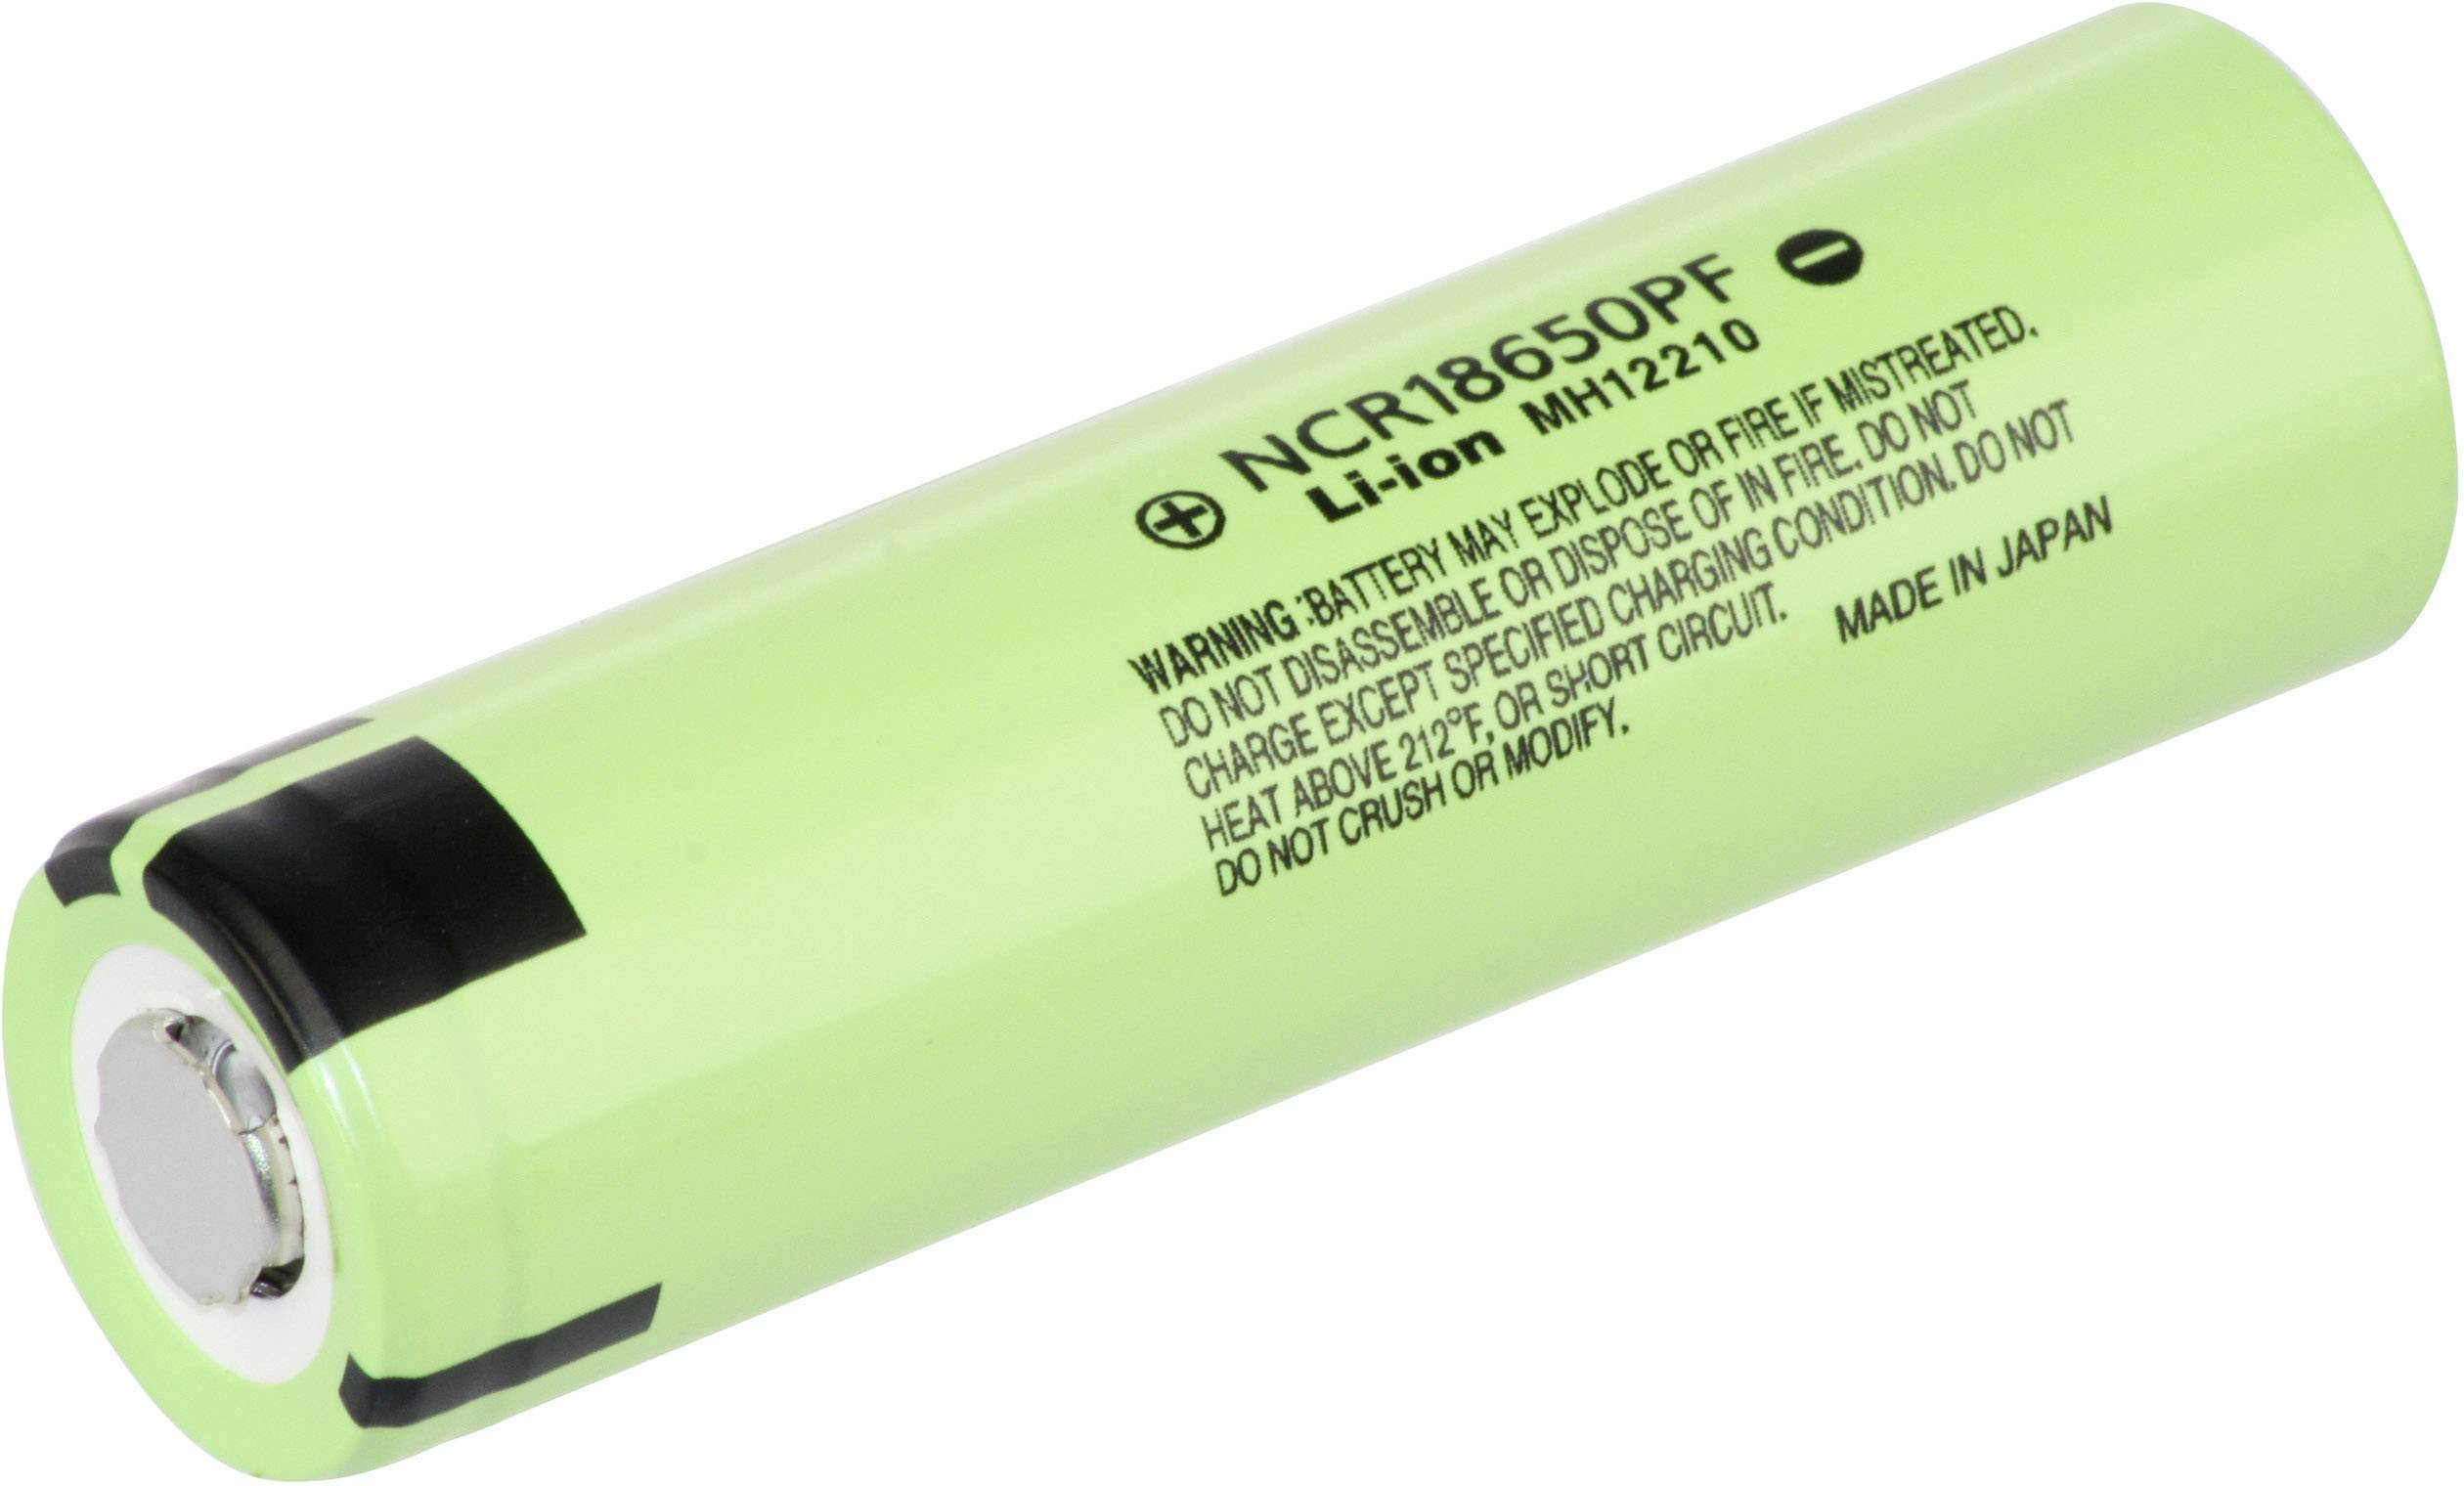
\includegraphics[width=0.45\linewidth]{images/18650}
	  \caption{Celda NCR18650PF}
	\end{minipage}
	\begin{minipage}{0.65\linewidth}
	  \begin{itemize}
		\item Capacidad: \\Min. 2750mAh | Max. 2900mAh
		\item Voltage nominal: 3.6V
		\item Carga: CC-CV, Std. 1375mA, 4.20V, 4.0 hrs
		\item Densidad energética: \\577Wh/l | 207 Wh/kg
	  \end{itemize}
	\end{minipage}
  \end{figure}

  \vspace{10pt}

  \begin{figure}[h!]
	\centering
	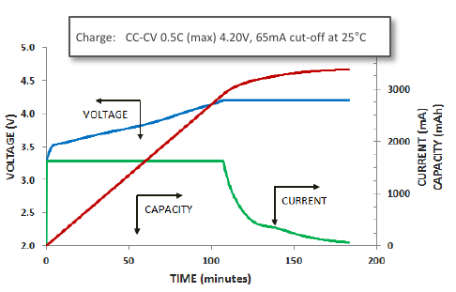
\includegraphics[width=.32\textwidth]{images/cc_cv_18650}\hfill
	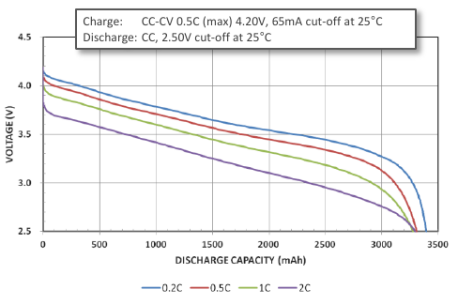
\includegraphics[width=.32\textwidth]{images/discharge_18650}\hfill
	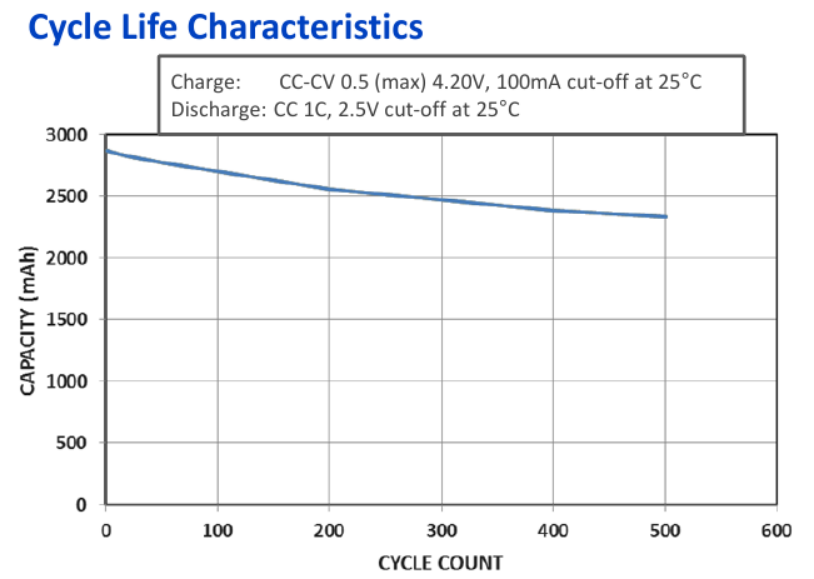
\includegraphics[width=.32\textwidth]{images/life_cycle_18650}
	\caption{Curvas características de la celda NCR18650PF}
  \end{figure}

\end{frame}

\section{Estimación del SoC}

\begin{frame}[allowframebreaks]
  \frametitle{Métodos de Estimación de SoC}

  Hoy en día hay varios métodos para estimar el Estado de Carga de una batería,
  entre ellas se encuentran las siguientes:
  \begin{itemize}
	\item Relación directa entre el SoC y el OCV
	\item Conteo de carga o, en inglés, \emph{Coulomb Counting}.
	\item Método por Fuerza Electro-Motriz.
	\item Resistencia Interna.
	\item \textbf{Estimación del Estado de Carga basado en modelos matemáticos.}
  \end{itemize}

  \framebreak

  Dentro del último, nos encontramos con los distintos modelos disponibles:

  \begin{itemize}
	\item Estimación basada en modelos Térmico y Electroquímicos.
	\item Modelo Eléctrico.
	  % TODO: Mover espectroscopía dieléctrica.
	\item Espectroscopía Dielétrica.
  \end{itemize}

  El error inherente de estos modelos puede ser compensado utilizando Filtros
  predictivos, como por ejemplo, un Filtro de Kalman con sus respectivas
  variaciones.

\end{frame}

\begin{frame}[allowframebreaks]
  \frametitle{Método de estimación por FEM}

  En este caso, se realiza la estimación del OCV mediante el estudio de la
  respuesta temporal de la tensión entre los terminales de la batería
  \emph{(fig. \ref{fig:relax_emf})} a través
  de una ecuación diferencial de primer órden \emph{(ec. \ref{ec_fem})}.

  \begin{minipage}{0.4\textwidth}
	\centering
	\begin{equation}
	  \frac{df(x)}{dx} = \alpha f(x)
	  \label{ec_fem}
	\end{equation}
  \end{minipage}
  \hspace{10pt}
  \begin{minipage}{0.4\textwidth}
	\begin{figure}[h!]
	  \includegraphics[width=1\textwidth]{images/EMF_relaxation.png}
	  \caption{Curva de relajación de una batería de Litio-Ion}
	  \label{fig:relax_emf}
	\end{figure}
  \end{minipage}

\end{frame}

\begin{frame}[allowframebreaks]
  \frametitle{Estimación basada en modelos Físicos}

  Este método requiere un profundo conocimiento de los fenómenos físicos y
  electroquímicos dentro de las baterías, como también la aplicación de las
  siguientes ecuaciones:

  \begin{itemize}
	\item Conservación de carga y masa en un sólido homogéneo.
	\item Conservación de carga y masa en un electrolito homogéneo.
	\item Ecuación de Butler-Volmer de movimiento de cargas en una unión entre
	  un sólido conductor y una solucion de Litio-Ion.
  \end{itemize}

\end{frame}

\begin{frame}[allowframebreaks]
  \frametitle{Estimación por resistencia interna}

  Se excita a la celda con un pulso de corriente de corta duración y se
  calcula la resistencia interna aplicando la ley de Ohm
  \emph{(eq. \ref{eq:ohm_law})}, obteniendo como resultado la gráfica de la
  Figura \ref{fig:r_ohm_result}

  \begin{minipage}{0.3\textwidth}
	\begin{equation}
	  \frac{\Delta V}{\Delta I} = R_\Omega
	  \label{eq:ohm_law}
	\end{equation}
  \end{minipage}
  \hspace{10pt}
  \begin{minipage}{0.55\textwidth}
	\begin{figure}[h!]
	  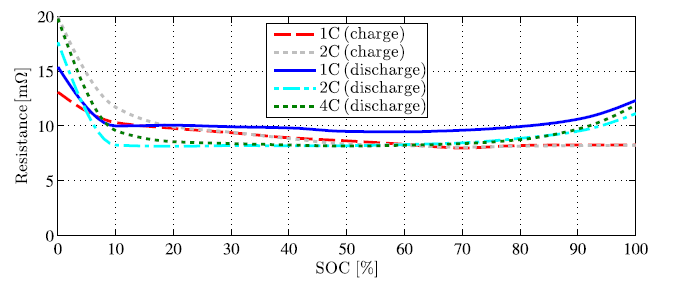
\includegraphics[width=1\textwidth]{./images/Ro_vs_SOC.png}
	  \caption{Resistencia Interna vs SOC de una batería}
	  \label{fig:r_ohm_result}
	\end{figure}
  \end{minipage}
\end{frame}

\begin{frame}[allowframebreaks]
  \frametitle{Espectroscopía Dielétrica (EIS)}
  Consiste en llevar a la celda en un estado de carga conocido y excitar los
  terminales con una onda senoidal de tensión o corriente, midiendo su respectiva
  respuesta. Un ejemplo de ella se puede observar en la Figura \ref{fig:nyq_eis}

  \begin{figure}[h!]
	\centering
	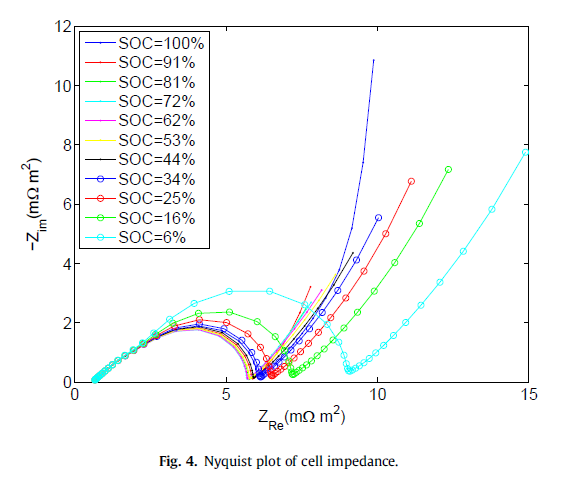
\includegraphics[width=0.5\textwidth]{./images/EIS_Nyquist.png}
	\caption{Espectroscopía Dielétrica de una batería Litio-Ion}
	\label{fig:nyq_eis}
  \end{figure}
\end{frame}

\begin{frame}[allowframebreaks]
  \frametitle{Filtro de Kalman}

  El filtro de Kalman es un algoritmo recursivo que corrige las estimaciones
  mediante la probabilidad conjunta de una o varias mediciones de un fenómeno y
  su estimación obtenida por modelos matemáticos.

  \begin{figure}[h!]
	\centering
	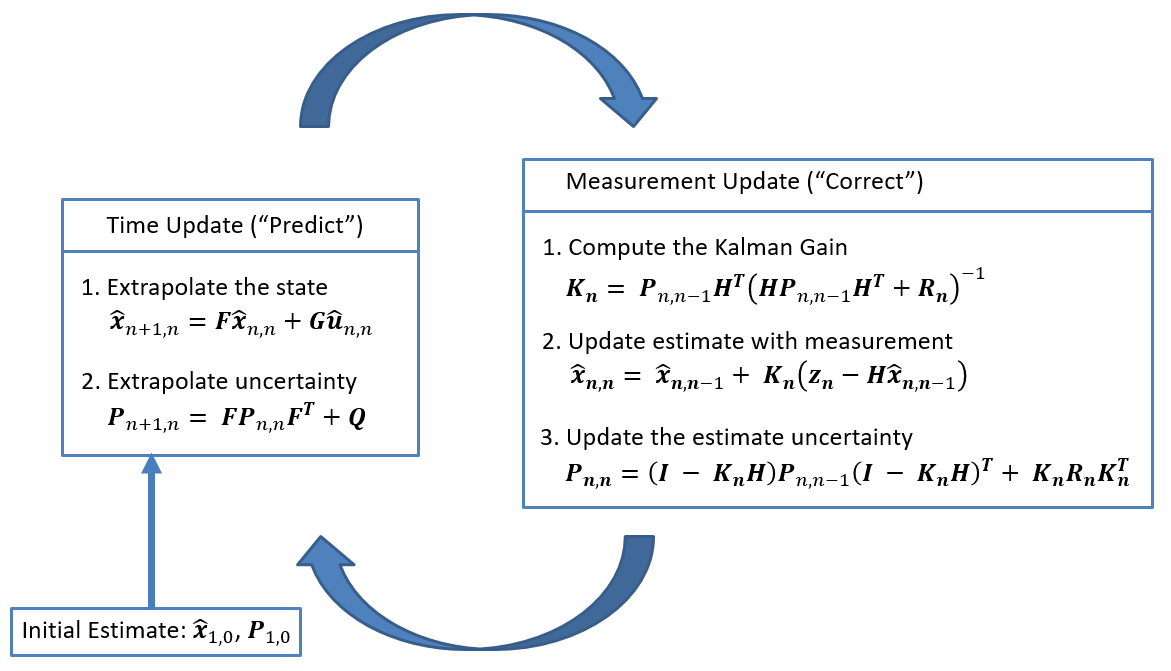
\includegraphics[width=0.7\textwidth]{images/KalmanFilterDiagram.png}
	\caption{Diagrama del Filtro de Kalman}
	\label{fig:kf_sch}
  \end{figure}

\end{frame}

\begin{frame}[allowframebreaks]
  \frametitle{Modelo Eléctrico + Filtro de Kalman}

  En este caso buscamos implementar un modelo eléctrico de una celda de
  Litio-Ion complementado con un Filtro de Kalman debido a que:

  \begin{itemize}
	\item Los componentes eléctricos de un modelo y sus dinámicas ya son de
	  nuestro conocimiento.
	\item Los cálculos de los parámetros del circuito son simples de estimar en
	  base a un set de datos.
	\item El Filtro de Kalman es un filtro predictor con amplia bibliografía y
	  ejemplos, lo que facilita su implementación.
	\item Nos permite extender el modelo a una implementación física con un
	  ajuste fino minimizando errores.
  \end{itemize}

\end{frame}

\section{Modelo equivalente}
\begin{frame}
  \frametitle{ Datos Experimentales}

	Como punto de partida, utilizamos un set de datos 
	%TODO: agregar referencia a bibtex del dataset
	de la Universidad de Wisconsin-Madison donde se realizó una serie de 
	ensayos sobre una celda NCR18650P. En la figura 
	\ref{fig:perfildeensayohppc}, se puede observar un ensayo HPPC sobre la 
	celda.

  \begin{figure}
	\centering
	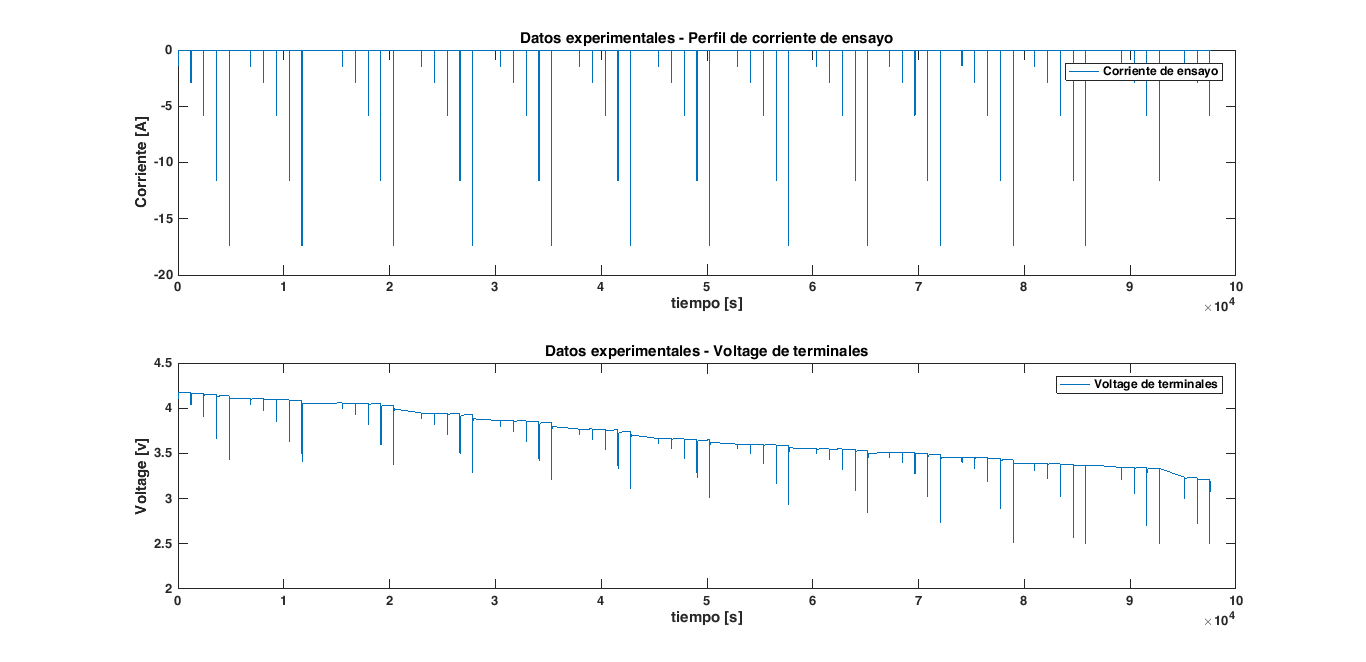
\includegraphics[width=1\linewidth]{images/HPPC-Completo}
	\caption{Perfil V-I de ensayo HPPC completo}
	\label{fig:perfildeensayohppc}
  \end{figure}

\end{frame}

\begin{frame}
  \frametitle{Modelo equivalente de una celda NCR18650PF}

  El modelo equivalente propuesto para replicar la dinámica de la celda a
  implementar se puede observar en la figura \ref{fig:ModeloBat}

  \begin{figure}

	\begin{center}
	  \ctikzset{bipoles/length=1cm}
	  \begin{circuitikz}[american]

		\draw (0,3) to[vsource, v=$V_{m}$](0,0);

		\draw (0,3) to [R = $R_{0}$](2,3);

		\draw (2,2.5)--(2,3.5);
		\draw (2,3.5) to [C=$C_{1}$] (4,3.5);
		\draw (2,2.5) to [R=$R_{1}$] (4,2.5);
		\draw (4,2.5)--(4,3.5);

		\draw (4,3) -- (5,3);

		\draw (5,2.5)--(5,3.5);
		\draw (5,3.5) to [C=$C_{2}$] (7,3.5);
		\draw (5,2.5) to [R=$R_{2}$] (7,2.5);
		\draw (7,2.5)--(7,3.5);

		\draw (7,3) -* (9,3);

		\draw (7,3) to[short,i^=$I$] (9,3)
		to[open,v^=$v_{term}$,o-o] (9,0)
		to[short] (0,0);

	  \end{circuitikz}



	  \caption{Modelo equivalente de una celda NCR18650B}
	  \label{fig:ModeloBat}
	\end{center}
  \end{figure}

\end{frame}

\begin{frame}
  \frametitle{Validación orden del modelo propuesto}

  Validamos el orden del modelo gráficamente ajustando y comparando una función 
  suma de exponenciales, como la observada en \ref{eq:exp2}, a la evolución del 
  voltaje en terminales de la bateria en su semi-periodo de relajación. De esta 
  forma comprobamos que el orden del modelo nos permite copiar tanto las 
  dinámicas rapidas como lentas de la batería. 

  \begin{equation}
	f(x) = a*e^{b*x} + c*e^{d*x}
	\label{eq:exp2}
  \end{equation}

  \begin{figure}
	\centering
	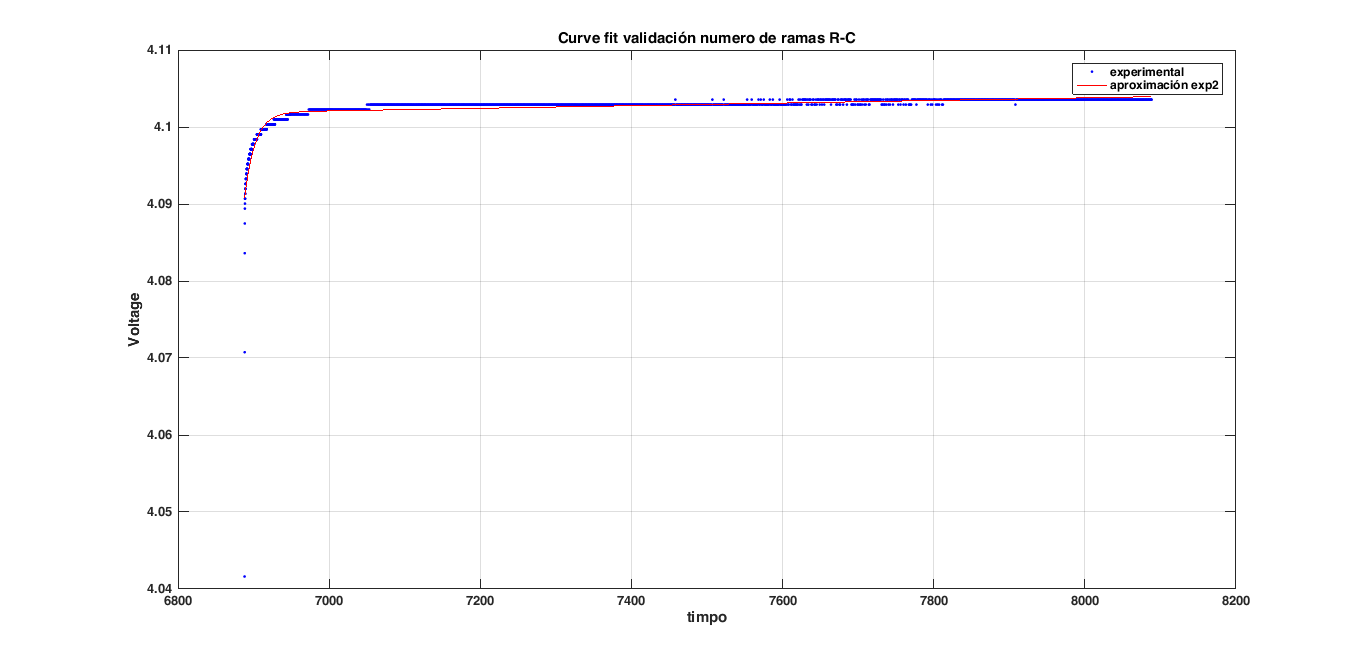
\includegraphics[width=0.9\linewidth]{images/exp_ord_2_val.png}
	\caption{}
	\label{fig:val_exp2}
  \end{figure}

\end{frame}


\begin{frame}[allowframebreaks]
  \frametitle{Estimación de parámetros del modelo}

  Implementamos en Matlab un estimador de parámetros RC del 
  modelo propuesto. Usamos el\emph{Estimador de parámetros} del Toolbox 
  Identificador de Sistemas de simulink.

  El método implementado es el de aproximaciones sucesivas a partir de comparar 
  los datos experimentales con los obtenidos a partir de la simulación de 
  simulink.

  \begin{figure}
	\centering
	\includegraphics[width=0.9\linewidth]{images/Modelo_celda_simulink.png}
	\caption{Modelo Simulink Simscape de celda  NCR18650B }
	\label{fig:simulink_celda}
  \end{figure}

  Fraccionamos los datos experimentales obtenidos del ensayo HPPC y calculamos 
  un juego de parámetros para cada escalon de corriente del ensayo asociado a 
  un SOC determinado.

  \begin{figure}
	\centering
	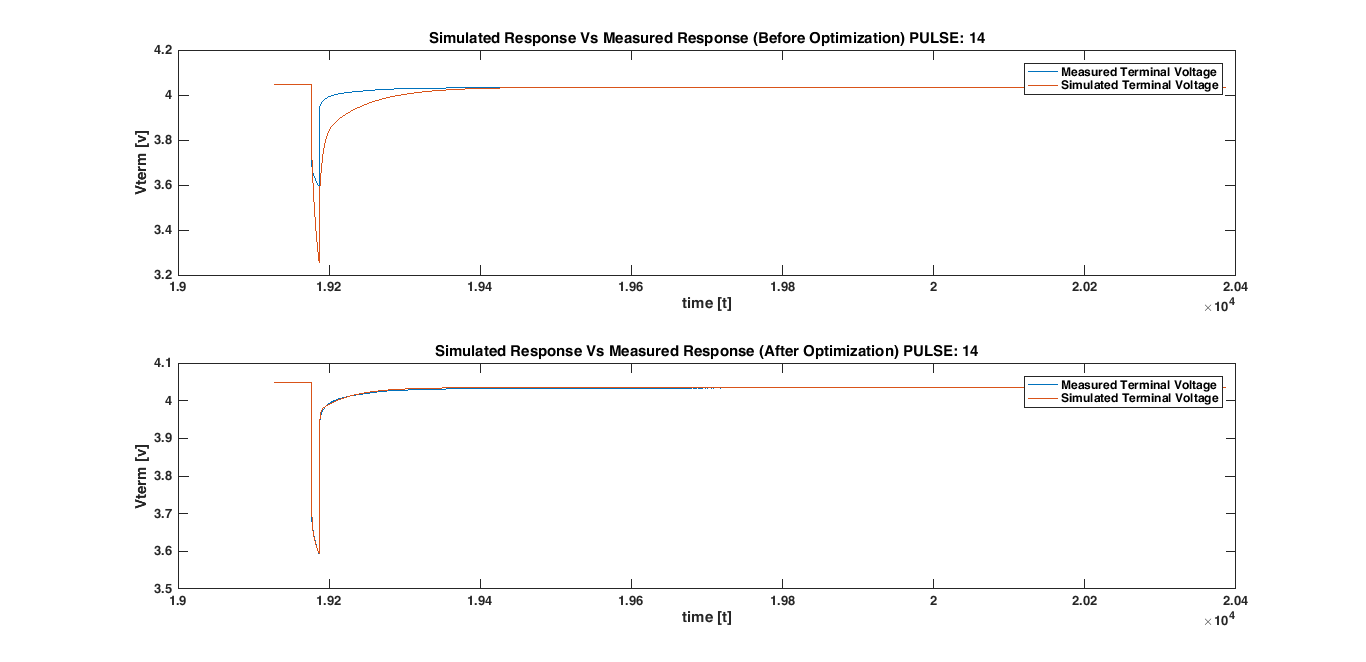
\includegraphics[width=0.9\linewidth]{images/Optimizacion.png}
	\caption{Resultado proceso Ajuste de parametros del modelo}
	\label{fig:RC_Opt}
  \end{figure}

  Obtuvimos un juego de 67 valores de cada elemento interno del modelo.

%TODO: Agregar imagen comparativa de Rs y Cs

  Corregimos los valores de los elementos calculados ensayando el modelo con un 
  perfil de corriente de un drive cicle y comparando los datos obtenidos con 
  los valores experimentales.

%TODO: Agregar imagen de comparación. 

\end{frame}

\begin{frame}[allowframebreaks]
	Después de obtener los parámetros del modelo, hicimos un ajuste fino para
	disminuir el error comparando los datos con los valores experimentales, como
	resultado obtuvimos las gráficas de la Figura \ref{fig:param_fine_tunning}.
\end{frame}

\end{document}
